\chapter{Convertitori A/D}
\section{Voltmetro Numerico}
Il \textbf{Voltmetro Numerico} è uno strumento che effettua misure di \textbf{tensione} mediante una \textbf{conversione analogico-digitale} della grandezza in ingresso e che visualizza il risultato numerico su un \textbf{display}:
\begin{center}
    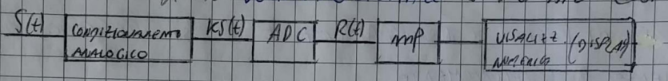
\includegraphics[width=\textwidth]{Images/figure25.png}
\end{center}
\begin{itemize}
    \item \textbf{Sezione di Condizionamento del Segnale in ingresso}, costituito da \textbf{partitori resistivi}, che ha il compito di amplificare/attenuare/filtrare il segnale per i blocchi successivi;
    \item \textbf{ADC} (Convertitore Analogico Digitale);
    \item \textbf{Microprocessore};
    \item \textbf{Display};
\end{itemize}
In particolare il \textbf{Convertitore Analogico Digitale} si può dividere in:
\begin{itemize}
    \item Convertitori \textbf{Istantanei};
    \item Convertitori ad \textbf{Integrazione};
\end{itemize}
Quelli \textbf{Istantanei} sono in genere più \textbf{veloci}, approssimando il segnale attraverso una\textbf{ serie di gradini}.\\ \\
Quelli ad \textbf{Integrazione} invece vengono usati per misurare \textbf{tensione continua} grazie alla loro elevata \textbf{reiezione al rumore }sovrapposto al segnale, tuttavia hanno un \textbf{tempo di conversione elevato}.
\section{Convertitore Multi Rampa}
\begin{center}
    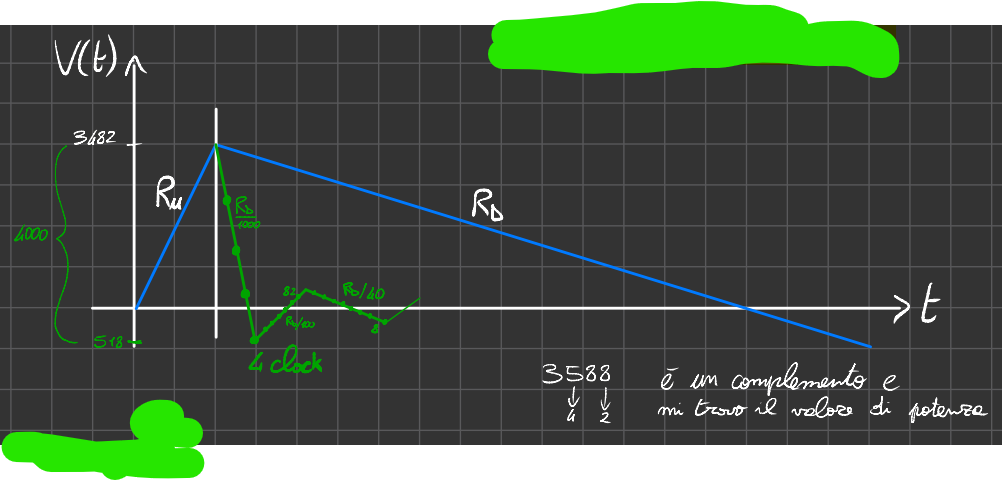
\includegraphics[width=.8\textwidth]{Images/figure46.png}
\end{center}
L'idea generale di questo \textbf{convertitore} è di fare una \textbf{serie di misure}, da prima \textbf{grossolane} e sempre via via più \textbf{precise}.

\section{Convertitore a Doppia Rampa}
Questo tipo di convertitore è utilizzato nel \textbf{multimetro} e consiste in una conversione \textbf{tensione/tempo}.\\ \\
Lo scherma a blocchi è costituito da:
\begin{itemize}
    \item Un \textbf{Integratore};
    \item Un \textbf{Comparatore di Zero};
    \item Un \textbf{Generatore di Tensione di Riferimento};
    \item Un Circuito per la \textbf{Misura dei Tempi}
\end{itemize}
\begin{center}
    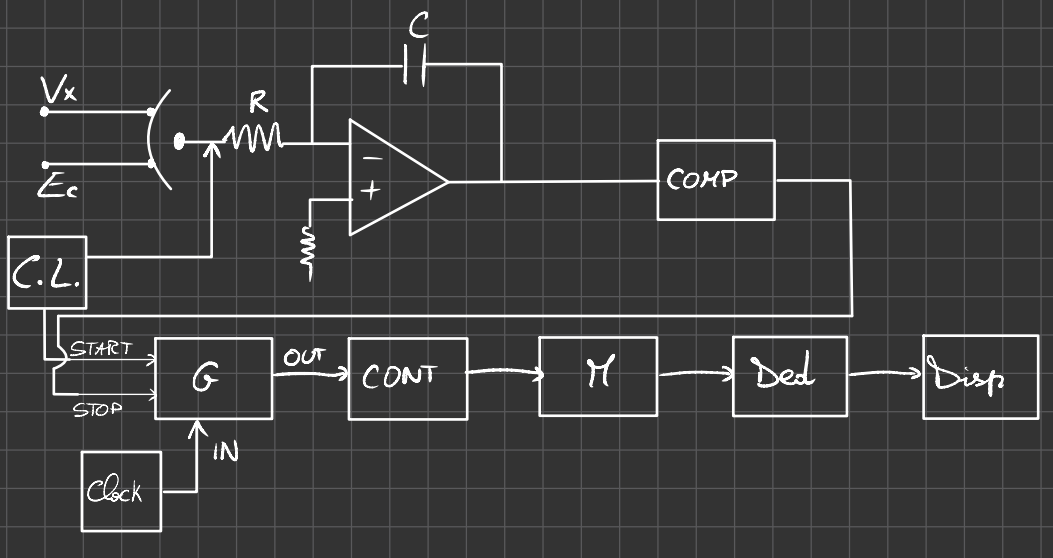
\includegraphics[width=\textwidth]{Images/figure27.png}
\end{center}

La misura avviene in due modi distinti:
\begin{itemize}
    \item Il segnale da misurare viene applicato all'ingresso del circuito e si inizia la \textbf{fase di conversione}; L'Integratore provvede ad \textbf{integrare} la tensione in ingresso per un \textbf{intervallo costante di tempo} ($T_{up}$);
    \item Dopo il tempo $T_{up}$, il \textbf{circuito di controllo} commuta l'ingresso dell'integratore verso una \textbf{tensione di riferimento} d'ampiezza nota e segno opposto alla tensione da misurare. A questo punto avviene una \textbf{seconda fase di integrazione} in cui la tensione si riduce a \textbf{zero}. Quando ciò avviene, il \textbf{comparatore} segnala il \textbf{passaggio per} \textbf{lo} \textbf{zero} e la Logica di Controllo interrompe il conteggio degli impulsi.
\end{itemize}
\begin{equation*}
    V_x = E_c \frac{T_{up}}{T_{down}}
\end{equation*}
\section{Convertitore ad Approssimazioni Successive}
\begin{center}
    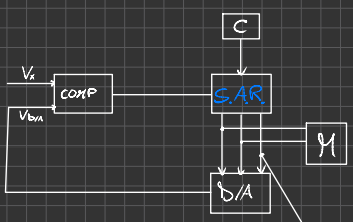
\includegraphics[width=.4\textwidth]{Images/figure42.png}
\end{center}
In questo dispositivo, un'opportuna catena di reazione fa \textbf{variare il D/A} fin quando non \textbf{eguaglia} la tensione del segnale analogico che si vuole misurare.\\
Il controllo del D/A avviene tramite un \textbf{registro di approssimazioni successive} (SAR) che pone a \textbf{1 il bit più significativo} (MSB).\\
Il \textbf{comparatore} confronta \textbf{l'uscita del D/A} con \textbf{l'ingresso analogico} e lo lascia ad 1 se D/A $<$ Ingresso oppure 0 se D/A $>$ ingresso. (\textbf{Ricerca in un albero di ricerca)}\\
Dopo N confronti, il \textbf{SAR} confronterà il valore numerico corrispondente all'ingresso analogico.
\section{Convertitore di Tipo parallelo (Flash)}
\begin{center}
    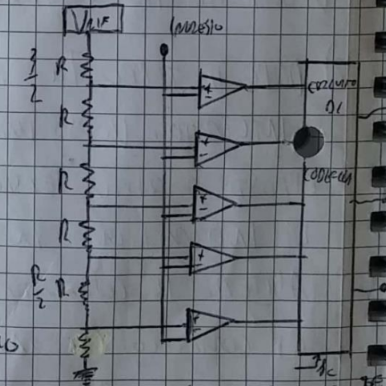
\includegraphics[width=.5\textwidth]{Images/figure45.png}
\end{center}
Questo convertitore è il più \textbf{veloce} tra quelli esistenti, esso è costituito da $2^n - 1$ \textbf{contatori} \textbf{analogici} che confrontano il segnale con $2^n -1$ valori diversi di \textbf{tensione} \textbf{di} \textbf{riferimento}.\\ \\
Il vantaggio maggiore è dovuto al fatto che tutti i \textbf{comparatori} eseguono il confronto nello \textbf{stesso} \textbf{istante}, riducendo il processo di \textbf{quantizzazione} ad un solo istante.\\ \\
Ci sono diverse sorgenti di \textbf{Errore}:
\begin{itemize}
    \item \textbf{Errori} \textbf{Statici} introdotti dai \textbf{comparatori} sia come tensioni di offset sia come correnti di offset e di bias;
    \item \textbf{Errori} dovuti alla \textbf{rete} \textbf{resistiva};
    \item \textbf{Errori} \textbf{Dinamici} dovuti ai \textbf{comparatori}
\end{itemize}

\section{Convertitore Serie Parallelo (Pipeline)}
\begin{center}
    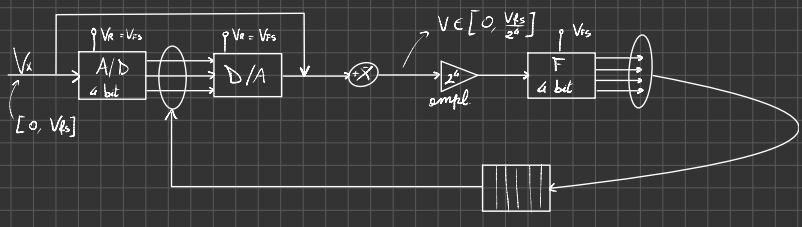
\includegraphics[width=\textwidth]{Images/figure39.png}
\end{center}
Il segnale di ingresso viene \textbf{convertito in digitale} in un primo stadio, \textbf{riconvertito in analogico} in un secondo e successivamente viene \textbf{sottratto} con se stesso.\\ \\
Il risultato è ottenuto dopo una moltiplicazione per $2^n$, quindi il risultato, composto dall'insieme dei bit ottenuti, dovrà essere \textbf{shiftato}.\\ 
Questa misura \textbf{dura un colpo di clock}.
